\chapter{Iso-Response Contours Provide a Geometric Interpretation of Neurons}

%%%% From paper
\section{Introduction}\label{intro}
%* Theories for how/why attacks happen
%- cascading linearity (goodfellow et al. 2015)
%- excessive invariance
%- subspace view
%- classication boundary curvature view
%- ford et all adv examples & noise
%    * adv examples are the nearest test error
%    * although our model doesn't have better test error, we argue that the nearest point is more data-aligned.
%    * We should also test against distribution shift (fig 7, right from their paper)
%    
%* Defense methods
%- supplementing the dataset with adversarial examples
%- augmenting loss function with adv loss (madry)
%- preprocessing / denoising images (although this is difficult to do without heavily reducing model performance)
%
%* Models that have relevance to ours:
%- sun et al (sparse coding, although they are also obfuscating gradients)
%- marzi et al (sparsity, although they are also obfuscating gradients)
%- DARCCC (population nonlienarity?)
%* Find more papers that look at adversarial images compared to the image manifold \parencite{sun2018adversarial}.

Adversarial examples are a demonstration of an ANN’s inability to cope with a distributional shift from its training data \parencite{ford2019adversarial}. They represent a worst-case demonstration of this weakness, which is a general problem that all classification ANNs are susceptible to \parencite{hendrycks2018benchmarking}. We postulate that designing machine learning algorithms that are both accurate and robust to adversarial attacks requires a radical reformulation in how such algorithms are currently constructed. In particular, we propose to abandon a strict reliance on reducing classification loss (i.e. an exclusive focus on classification accuracy) and instead allow our models to undergo a period of unsupervised learning that mimics the cognitive development of biological nervous systems. Biological systems are robust to adversarial examples that affect deep networks. However, in time-limited regimes that result in predominantly feed-forward brain computation adversarial attacks have been shown to influence human decision making \parencite{elsayed2018adversarial}, suggesting that slower recurrent feedback loops aid in adversarial robustness. Furthermore, congruent with current theories for probabilistic inference in the brain \parencite{lee2003hierarchical}, we augment the standard ANN architecture with lateral connectivity and recurrence. We propose that, together, these innovations will improve the network’s specificity to signals that lie along the data manifold. We use adversarial attacks as a mechanism for understanding both traditional pointwise nonlinear ANNs and a population nonlinear alternative.

Adversarial attacks represent a recently discovered flaw in typical deep neural networks, where small targeted perturbations in the input space can cause large undesired changes in the output space. Although the discovery of adversarial examples in deep networks is relatively new, a fervor of research has produced a large body of literature on the subject and an understanding of these attacks has begun to emerge. In the pioneering work of Szegedy et al. \citeyearpar{szegedy2013intriguing}, they introduce the idea of ``adversarial attacks'' for deep networks and propose that a non-smooth decision boundary in classification networks produces adversarial ``pockets'' interspersed among dataset examples. They also suggest that adversarial images represent a counter-example to the hypothesis that deep networks are able to achieve local generalization to input space regions in the vicinity of training examples. Although this latter hypothesis has continued to hold, the presence of universal and transferable adversarial directions \parencite{moosavi2017universal} suggests that there are not adversarial pockets in the input manifold. The follow up work of Goodfellow et al. \citeyearpar{goodfellow2014explaining} make several proposals, some of which have been refuted \parencite{jetley2018friends}. However, we would like to emphasize two important arguments from their work: 1) they present evidence suggesting that the direction of perturbation is more important than the specific point in space (further refuting the ``pockets'' theory), and 2) the adversarial perturbations are highly aligned with the weight vectors of a model. The last of those observations has been explored in much more detail by Jetley et al. \citeyearpar{jetley2018friends}, who suggest that deep networks produce classification boundaries based on a small number of features that correspond to high curvature directions in the input space and that these high curvature directions are also the most effective adversarial directions. The works of Gilmer et al. \citeyearpar{gilmer2018adversarial} and Ford et al. \citeyearpar{ford2019adversarial} further expand on this idea by suggesting that adversarial attacks confined to the $l_{\infty}$ box represent the worst-case example of the model's inability to account for distributional shift generally. However, the works of Kos et al. \citeyearpar{ford2019adversarial} and Goodfellow et al. \citeyearpar{goodfellow2014explaining} demonstrate the ability to produce adversarial examples for pointwise-nonlinear generative models that have applications in image denoising, suggesting a more nuanced explanation of adversarial susceptibility. Recent work has also shown that nearly all proposed adversarial defense mechanisms fail in the face of more careful attacks \parencite{carlini2017towards, athalye2018obfuscated}.  For example, the recent defense method proposed by \parencite{sun2018adversarial} claims to produce an adversarially robust preprocessing step, although they use basis pursuit in their methods, which possibly achieves robustness through gradient obfuscation \parencite{athalye2018obfuscated}. However, their intuition that images should be forced onto the image manifold as a preprocessing step has great relevance to the work herein. It will always be possible to produce an image perturbation that results in a change in class label, or an alternate reconstruction. The academic fascination in the subject comes from observations of how small that perturbation needs to be and the (lack of) semantic content of the perturbation. Following the intuition provided in \parencite{ford2019adversarial}, successful defenses appear to require accomplishing one of two goals: 1) robustly denoising inputs to prevent distributional shift or 2) training deep networks to be more robust to worst-case distributional shift.

Inferring causes from natural signals is a challenging problem faced by biological vision systems. For artificial vision, the neural network community has largely tackled this problem using feedforward discriminative models. An alternative approach is to use generative models, in which the network must attempt to explain data in terms of an internal model of the world. In BNNs we see a preponderance of evidence that individual neurons are highly non-linear, recurrent, and laterally connected. The Locally Competitive Algorithm (LCA) \parencite{rozell2008sparse} is a generative sparse coding model that represents an example of how lateral inhibition can be derived from a well-defined computational objective. This network has been shown previously to exhibit a variety of non-linear receptive field effects \parencite{zhu2013visual}. Many of these effects can be explained using the model neuron’s iso-response contours - a common experimental method in neuroscience for determining stimulus combinations that result in equal activation from recorded neurons \parencite{golden2016conjectures}. In the brain, the atomic unit of computation is generally considered to be the neuron, but most deep learning research has eschewed the individual neuron, possibly obfuscating the connections between BNNs and ANNs. We propose to adopt the single-neuron iso-response analysis to better understand adversarial attacks on ANNs while varying degrees of biological realism.

To better understand how adversarial attacks differ for BNNs and ANNs, we compared feed-forward, pointwise nonlinear discriminative and generative network architectures against more biologically informed population nonlinear generative network architectures. Pointwise nonlinearities are the more traditional form of nonlinearities, as seen in nearly all deep neural network architectures. They are defined as nonlinearities that are a function of only a single neuron in a layer and include rectification, sigmoid, and hyperbolic tangent. Population nonlinearities represent the alternative class, where the nonlinearity output is a function of multiple neurons in a set. These include softmax, divisive normalization \parencite{carandini2012normalization, balle2016end} and the network nonlinearity present in sparse coding \parencite{rozell2008sparse, olshausen1997sparse}. In principle, generative models should not be as susceptible to adversarial attacks as discriminative models because they are trying to fit their internal model to the data as a ``sanity check'', which should not succeed for adversarial perturbations. One method by which generative models can perform such a sanity check is via recurrent maximum a-posteriori (MAP) inference. The LCA network uses population nonlinear interactions via lateral connectivity among neurons to facilitate this process, resulting in an ``explaining away'' effect commonly referenced in Bayesian inference literature \parencite{olshausen2014perception, citation}.

Here, drawing from the architecture and function of brains, we propose that a network with lateral inhibitory connectivity in its hidden layer forces adversarial perturbation vectors to have angles that are more in line with data dimensions, producing more semantically meaningful perturbations. We develop an analytic argument to support this claim for untargeted adversarial attacks. Furthermore, we demonstrate by experiment that our method successfully improves robustness to adversarial attacks and more broadly distributional shift for a classifier trained on our model's outputs. The contribution of our work is a novel perspective for understanding adversarial attacks and population nonlinear networks. We also demonstrate that simple generative models can be used to improve a typical network’s defenses against adversarial attacks.

\section{Neuron response geometry explains adversarial robustness}\label{neuron}
We propose to perform single neuron and population level analysis by extending the iso-response contour theory to be used as a lens to understand untargeted adversarial perturbations for individual neurons. Additionally, we have scaled up the iso-response analysis to models trained on images of handwritten digits (MNIST, \parencite{citation}) and natural scenes (CIFAR, \parencite{citation}). We show that the response geometry of LCA neurons predicts data-aligned perturbations when attacking the entire network, resulting in semantically meaningful adversarial attacks. We provide a theoretical argument to support this intuition by exploring the iso-response contours and orthogonal adversarial directions for individual neurons and give empirical evidence to further bolster the claims. 

Biological neurons are highly interconnected, both across and within layers. This interconnection gives rise to strong population nonlinear effects. However, nearly all work in neuron modeling uses pointwise nonlinearities due to the ease in interpretation and implementation. Work from \citeyearpar{golden2016conjectures} suggests a novel single-neuron analysis technique that allows us to increase the complexity of our neuron models without decreasing our understanding by looking at the neuron’s response geometry. We extend this technique to larger scale models that allows us to predict important properties about the model’s susceptibility to adversarial attacks. We then analyze the attacks themselves to demonstrate how the single-neuron analysis extends to networks. We conduct our preliminary experimentation on two types of networks: those with pointwise nonlinearities and those with population nonlinearities (Figure \ref{fig:pointpopnets}). Although there are many types of networks that fit into these two categories, we reserve comparative analysis among them to future work and focus this study on two specific instances: Feedforward Autoencoders (AEs) and the Locally Competitive Algorithm (LCA). We focus on the LCA as the population nonlinear network because it has been shown to exhibit many linear and nonlinear response properties that are well matched to what is observed in the brain \parencite{zhu2013visual, olshausen1997sparse}. The LCA was first proposed by Rozell et al. \citeyearpar{rozell2008sparse} to perform sparse coding. It is a generative network that uses MAP estimates of data likelihood to build an internal model. It can also be thought of as an auto-encoder with a single recurrent hidden layer. Details on these models can be found in section \ref{sec:models}.

\subsection{Adversarial examples are orthogonal to iso-response contours}
To better understand the difference between population and pointwise nonlinearities, we visualize the input-output maps of model neurons in the form of iso-response contours (Figure \ref{fig:iso_contours}, see caption for more details). Golden et al. \citeyearpar{golden2016conjectures} used iso-response contours to explain several non-linear properties as well as variance/invariance properties for simple and complex cells. To construct the visualization, we consider a two-dimensional slice, or projection, in the high dimensional input space. We use each point (i.e. image) in the slice as input to the neuron model and bin the points according to the neuron's output amplitude (Figure \ref{fig:iso_contours}). The iso-response contours of linear neurons are straight: any input perturbation that is orthogonal to the weight vector will result in equal activation. For pointwise nonlinearities, this remains true: because the nonlinearity is performed after a linear projection, the output must also produce straight iso-response contours. By contrast, for a population nonlinearity the gradient of the activation function with respect to a small perturbation in the input is a function of all other neurons in the layer. Thus, for a perturbation that is orthogonal to a target neuron, it is highly likely that an alternative neuron will have a non-orthogonal weight vector, which will result in a net change in all neuron outputs. Therefore, iso-response contours for population nonlinear neurons can be bent.

Adversarial examples are closely tied to neuron iso-response contours. While an iso-response contour represents a perturbation direction in stimulus space that produces no change in the output, an adversarial example is a perturbation direction that produces a maximal change in the output. Below, we present analytic arguments that these two response directions are orthogonal for individual neurons.

If we extend the work of Marzi et al. \citeyearpar{marzi2018sparsity} to include nonlinear functions, then we can define adversaries as seeking to maximize the following measure, $\Delta$, with respect to a perturbation, $e$:

\begin{align}\label{eq:adv_metric}
\begin{split}
    \max_{e} \Delta (s, s+e) = \max_{e} |f(s+e) - f(s)| \\
    s.t. \|e\|_{\infty} < \varepsilon,
\end{split}
\end{align}
where $f()$ can include a non-linear activation function, $s$ and $e$ are equal sized column vectors representing the data and perturbation, respectively, and $\varepsilon$ is some small scalar value. To solve this equation, one must find a perturbation that results in a model output that is maximally different from the output with respect to the original input. For our analysis, $e$ indicates a targeted perturbation of fixed magnitude that is subject to $|e|_{\infty}<\varepsilon$. By definition, for any vectors $u$ and $v$, $\langle u,v\rangle = |u| \cdot |v| \cdot cos(\Theta_{u,v})$. Going forward, we will reference the inner angle between two vectors as $\Theta_{u,v}$ for some vectors $u$ , $v$. If we assume that the perturbation magnitudes are fixed and equal, i.e.$|e_{adv}| = |e_{iso}| = k < \varepsilon$, then we can optimize over the angle between the perturbation vector and the input signal $\Theta{e,s}$. We can now include perturbation directions that result in a minimal change in the neuron's output:

\begin{center}
    \begin{tabular}{ |c | c| } \hline
     \textbf{Adversarial} & \textbf{Iso-Response} \\ \hline
     $\max_{\Theta_{e,s}}|f(s+e) - f(s)|$ & $\min_{\Theta_{e,s}} | f(s+e) - f(s) |$ \\ \hline
    \end{tabular}
\end{center}

These so called ``iso-response'' directions create contours in the neuron's response field. We can use the Fr\'{e}chet derivative \parencite{citation} to better understand how the neural response geometry relates to adversarial images:

\begin{align}\label{eq:frechet}
\begin{split}
    f(s+\varepsilon) &= f(s) + \langle\nabla_{s}f(s), \varepsilon\rangle + o(\varepsilon)\\
    &\therefore \\
    f(s+\varepsilon) - f(s) &= \langle\nabla_{s}f(s), \varepsilon\rangle+ o(\varepsilon),
\end{split}
\end{align}

where $\langle , \rangle$ indicates a dot product and $o(\varepsilon)$ is a tight bound that means ''terms that are, in the limit $\varepsilon \rightarrow 0$, dominated by $\varepsilon$\". Combining this with the bottom equality in equation \ref{eq:frechet} gives us:

\begin{align}\label{eq:angle_metric}
\begin{split}
    &\textbf{Adversarial:} \max_{\Theta_{e,s}} |f^{\prime}(s)^\top e + o(\|e\|)|,\\
    &\textbf{Iso-Response:} \min_{\Theta_{e,s}} |f^{\prime}(s)^\top e + o(\|e\|)|,
\end{split}
\end{align}

where $f^{\prime}(s) = \nabla_{s}f(s)$ is the output gradient of the target neuron. For small $\|e\|$, the linear terms in equation \ref{eq:angle_metric} dominate and these equations are solved when $e \parallel f^{\prime}(s)$ for the adversarial perturbation and $e \perp f^{\prime}(s)$ for the iso-response perturbation. This tells us that the optimal adversarial directions will always be perpendicular to the iso-response directions for an untargeted adversarial attack. 

\subsection{Iso-response contours}
Although we cannot analytically estimate the shape of the iso-response contours for population nonlinear neurons, we know that the adversarial directions will be perpendicular to them. Therefore, we can estimate adversarial perturbation directions by measuring the iso-response contours empirically. Figure \ref{fig:adv_grads} shows schematic drawings of the contours measured for population- and pointwise-nonlinear neurons along with the expected adversarial directions.

The response function of a model neuron for a perturbation, $e$, added to an input signal, $s$, can give us insight to that neuron's iso- and adversarial-response properties. First, we will describe this for a linear neuron, $a_{k}=f_{k}(s)=\phi_{k}^\top s$:

\begin{align}\label{eq:linear_neuron}
\begin{split}
    a_{k}(s+e) &= f_{k}(s+e) = \phi_{k}^\top (s + e) \\
    &= \phi_{k}^\top s +\phi_{k}^\top e,
\end{split}
\end{align}

where $\phi_{k}$ is a column weight vector. Next we match equation \ref{eq:linear_neuron} to the top part of equation \ref{eq:frechet}:

\begin{equation}
    f(s) + \langle\nabla_{s}f(s), e\rangle + o(\|e\|) = \phi_{k}^\top s + \phi_{k}^\top e.
\end{equation}

This tells us that the first term on the right hand side is $f(s)$ and the second term is $\langle\nabla_{s}f(s)^\top, e\rangle$, which means the third term is $o(||e||)=0$ (this is expected because it is a linear function). Therefore,  $\nabla_{s}f(s) = \phi_{k}$ and for any $e \perp \phi_{k}$, $f_{k}(s+e) = f_{k}(s)$. To summarize, for linear neurons:

\begin{align}\label{eq:parallel_adv_proof}
\begin{split}
    f(s) &= \phi_{k}^\top s \\
    f(s+e) &= \phi_{k}^\top s + \phi_{k}^\top e \\
    &\forall ||e||_{\infty} < \varepsilon \\
    &\therefore \\
    \max_{e} | f(s+e) - f(s) | &= \max_{e} | \phi_{k}^\top e | \\
    & \forall ||e||_{\infty} < \varepsilon
\end{split}
\end{align}

For a fixed amplitude perturbation, the maximum adversarial direction is when the inner angle $\Theta_{\phi_{k},e} = 0$. Additionally, perturbations that are orthogonal to $\phi_{k}$ are iso-response directions because they do not result in a change in $a_{k}$, which is illustrated in the top left plot of Figure \ref{fig:iso_contours}.

We can again use equation \ref{eq:frechet} to gain insight about the iso-response directions and adversarial directions for pointwise nonlinear functions, such that $a_{k}(s) = f_{k}(s) = g_{k}(\phi_{k}^\top s)$:

\begin{align}\label{eq:pw_nonlin}
\begin{split}
  a_{k}(s+e) &= g_{k}(\phi_{k}^\top(s+e)) \\
  &=g_{k}(\phi_{k}^\top s + \phi_{k}^\top e) \\
\end{split}
\end{align}

where $g_{k}(\cdot)$ is a pointwise non-linear activation function for neuron $k$. If we perform a change of variables such that $a = \phi_{k}^\top s$ and $b = \phi_{k}^\top e$, then we can fit equation \ref{eq:pw_nonlin} to match equation \ref{eq:frechet}:

\begin{align}\label{eq:pw_nonlin_frechet}
\begin{split}
    g_{k}(a + b) &= g_{k}(a) + \nabla_{s}g_{k}(a) \cdot b + o(b) \\
    &=g_{k}(\phi_{k}^\top s) + \nabla_{s}g_{k}(\phi_{k}^\top s) \cdot \phi_{k}^\top e + o(\phi_{k}^\top e)\\
    &=g_{k}(\phi_{k}^\top s) + \langle\nabla_{s}g_{k}(\phi_{k}^\top s) \cdot \phi_{k}^\top, e\rangle + o(\|e\|),
\end{split}
\end{align}

where $\cdot$ indicates pointwise vector multiplication. Now we match equation \ref{eq:pw_nonlin_frechet} to the bottom part of equation \ref{eq:frechet} to show 

\begin{equation}
\begin{split}
    |a_{k}(s+e) - a_{k}(s)| = |\nabla_{s}g_{k}(\phi_{k}^\top s) \cdot \phi_{k}^\top e + o(\|e\|)|.
\end{split}
\end{equation}

Again, the function is maximized when $\Theta_{\phi_{k}, e}=0$ and minimized when $\Theta_{\phi_{k}, e}=\tfrac{\pi}{2}$, which tells us that a pointwise nonlinearity can only change the spacing between the contours, it cannot bend the contours in any way.

Finally, we extend this analysis to population nonlinear networks. For population nonlinear networks, the output is now a function of the the other neurons in the layer as well as the input. Thus, $\Phi$ represents the entire weight matrix, with rows set to $\phi_{k}^\top$. We want to know how a small perturbation in the input changes \emph{all} of the outputs. We answer this by defining the activation gradient as:

\begin{align}\label{eq:pop_nonlinear}
\begin{split}
   a_{k}(s+e) &= p_{k}^\top g(\Phi(s+e)) \\
   &= p_{k}^\top g(\Phi s + \Phi e) \\
   &= p_{k}^\top g(\Phi s) + (\nabla_{s}g(\Phi s)^\top p_{k})^\top \Phi e + o(\|\Phi e\|) \\
   &= p_{k}^\top g(\Phi s) + (\Phi^\top \nabla_{s}g(\Phi s)^\top p_{k})^\top e + o(\|e\|),
\end{split}
\end{align}

where $p_{k}^\top$ is a one-hot vector selecting output $k$, $g(\cdot)$ is a function of all of the weight vectors and the input, and $\nabla_{s}g(\Phi s)$ is a Jacobian. We can no longer simply describe the contours of these neurons because the gradient of the non-linearity is now a function of (an arbitrary linear transformation of) $s$. For individual neurons, the contours can be straight or bent, and if bent they can bend towards the origin (endo-origin) or away from it (exo-orogin).

\begin{figure}[h]
%\vskip -0.05in
\begin{center}
\centerline{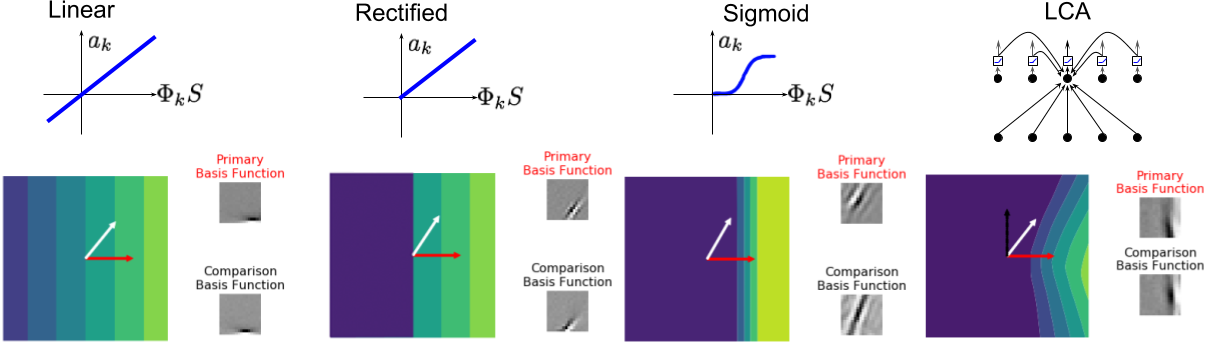
\includegraphics[width=\columnwidth]{Figures/iso_contour_comparison.png}}
\end{center}
%\vskip -0.3in
\caption{Empirically measured iso-response contours. A fine sampling of points in the 2D plane are injected into the high dimensional image space and used as inputs to a target model neuron, $a_{k}$. The color value indicates a binned normalized response magnitude of the neuron. The red arrow is the weight vector for the neuron, $\phi_{k}$. The white arrow is an alternate neuron's weight vector.}
\label{fig:iso_contours}
\end{figure}

%A histogram of 2nd order coefficients for polynomial fits to the lines in the middle plot. Negative coefficients indicate exo-origin curvature, which tells us that this neuron exhibits exo-origin curvature in all orthogonal directions tested.

\subsection{Population nonlinear neurons can be more robust to adversarial examples}
It is important to determine the shape of an individual neuron’s response contours for a large number of planes to better understand its high-dimensional geometry.  To do this, we used two different methods for choosing image planes. For both methods, we defined the horizontal axis as the weight vector (or basis function) for the target neuron. For the first method, we found a set of random vectors that are orthogonal to our target neuron’s weight vector and compute curvature in each plane. For the second method we start by finding another neuron’s weight vector that has a nonzero inner-product with our target neuron’s weight vector (and thus they are not orthogonal). Next, we used the Gram-Schmidt process to find a vector that is orthogonal to our target neuron, but coplanar with our second neuron. This method will increase the likelihood of competition between neurons, and thus increases the curvature. The result is shown in Figure \ref{fig:figure} and indicates that the neuron’s high-dimensional iso-response geometry is cone shaped, with negative curvature in every direction.

\begin{figure}[h]
%\vskip -0.05in
\begin{center}
\centerline{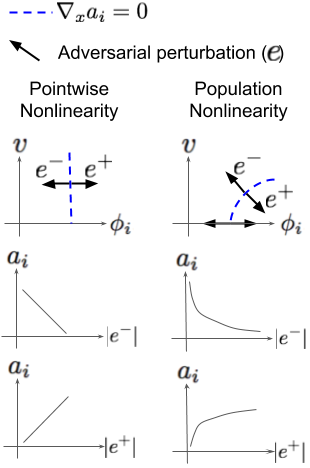
\includegraphics[width=0.5\columnwidth]{Figures/adversarial_gradients_iso_contours.png}}
\end{center}
%\vskip -0.3in
\caption{Adversarial gradients (dark arrows) are always orthogonal to the iso-response contours (blue dashed line).$\Phi_{k}$ indicates a weight vector for the neuron $a_{k}$, and $v$ represents a random orthogonal direction.}
\label{fig:adv_grads}
\end{figure}

Recall that the adversarial objective in equation \ref{eq:adv_metric} has an absolute value and is thus bi-directional. For a locally linear approximation of an untargeted attack, these two directions are equal. However, if we impose a rectifying constraint on our neuron outputs, then the two solutions are not equal for an individual neuron. For a sufficiently large $e$, the direction that lowers $a_{k}$ to below threshold will result in $f(s+e)=0$, i.e. $\max_{e^{-}}|f(s+e)-f(s)| = f(s)$. In other words, for rectified units, $\max_{e^{-}}|f(s+e)-f(s)|$ could be less than $\max_{e^{+}}|f(s+e)-f(s)|$. This would not be known to a simple gradient method for computing an non-targeted adversarial attack, such as that proposed in equation \ref{eq:adv_metric}. However, in practice actual adversarial attacks have an additional goal in mind: to produce an output that is reasonable for some \emph{other} data sample. Turning off all of the units in a layer is not a solution to this problem, so some set of adversarial perturbations must be in the $e^{+}$ direction. By definition, these perturbations will have greater contribution to the model's output than $e^{-}$ perturbations.

The Locally Competitive Algorithm (LCA) is a neural network with population nonlinearities that exhibits exo-origin bent iso-response contours. If the LCA is also rectified, then the $e^{-}$ direction will eventually turn off units. From Figure \ref{fig:adv_grads} one can deduce that the only $e^{+}$ direction that will cause $a_{k}$ to grow without bound is along $\Phi_{k}$. What's more, \emph{all} directions that increase $a_{k}$ are towards, or along, $\Phi_{k}$. From this analysis we present three hypotheses:

\begin{itemize}
  \item Adversarial attacks on networks with exo-origin bent contours will be more aligned with the their weight vectors than attacks on networks with straight contours. If the weight vectors are data aligned then this will result in adversarial attacks that are data aligned.
  \item Rectified LCA should be resistant to unbounded adversarial attacks.
  \item Non-rectified LCA should be more susceptible to adversarial attacks than rectified LCA.
  \item More overcompleteness causes more bending of the iso-response contours \parencite{golden2016conjectures}, which will result in better adversarial defense.
\end{itemize}

In the following section we will outline several models used for our experiments as well as the experiments performed. Then we will present results that support the above hypotheses. Finally we will discuss the implications of these results and propose continued directions for research.

\section{Experimental models}\label{sec:models}
\subsection{The Locally Competitive Algorithm} \label{sec:lca}
The Locally Competitive Algorithm finds a solution to the following optimization problem:

\begin{equation}\label{eq:energyfunc}
    \argmin\limits_{a}
        \left( E =
            \overbrace{ \tfrac{1}{2} \| s - a \Phi^{\top} \|_{2}^{2} }^\text{Preserve Information} +
        \overbrace{ \lambda \sum\limits_{i=1}^{M}C(a_{i}) }^\text{Limit Activations} \right),
\end{equation}

where $s$ is an input vector, $a$ is a neural activity vector, $\Phi$ is a weight matrix, and $C(\cdot)$ is a cost function on the activations, which will be the $l_{1}$ norm of the activity vector for our preliminary study: $C(a_{k}) = |a_{k}|$. The cost function has a considerable impact on the network dynamics \parencite{rozell2008sparse} and alternatives are of interest for future work. The LCA describes an activation coefficient, $a_{k}$, as the thresholded output of a model neuron's internal state, $u_{k}$. The network finds a minima to equation \ref{eq:energyfunc} by following its gradient:

\begin{displaymath}
    \dot{u_{k}}(t) &\propto - \frac{\partial E(t)} {\partial a_{k}(t)}
\end{displaymath}

\begin{equation}\label{udot}
    \dot{u_{k}}(t) &= \frac{1}{\tau} \left[\Phi^{\top}_{k}s - \sum_{m \neq k}^{M}G_{k,m}a_{m}(t) - f_{\lambda}(a_{k}(t)) \right],
\end{equation}

where $\tau$ is a time constant, $G = \Phi^T\Phi$, and $f_{\lambda}(a_{k}(t)) = a_{k}(t) + \lambda \frac{\partial C(a_{k}(t))}{\partial a_{k}(t)}$. A neuron's output is computed using a thresholding function $a_{k}(t) = T_{\lambda}(u_{k}(t)) = \text{ReLU}(f_{\lambda}^{-1}(u_{k}(t)))$:

\begin{equation}\label{lcathresholdfunc}
    T_{\lambda}(u_{k}(t)) = \left\{
    \begin{aligned}
        u_{k}(t)-\lambda,\;\; &u_{k}(t)\; >\; \lambda \\
        0,\;\; &u_{k}(t)\; <\; \lambda
    \end{aligned}
    \right.
\end{equation}

Our model differs from the original citation in that we rectify our output thresholding function. Finally, we can update our weights using stochastic gradient descent for a given sparse code of a batch of inputs:

\begin{equation}\label{phiupdate}
  \Delta \Phi = \eta (s - a(t=T)\Phi^{\top})^{\top} a(t=T),
\end{equation}

where $T$ is the total number of inference steps.

We suggest that the LCA requires stronger adversarial perturbation magnitudes to achieve the same change in the network output when compared to more standard feedforward autoencoders. Additionally, adversarial perturbations for the LCA are more aligned with the data than those for the alternative models tested. We have shown that both of these properties can be explained by an LCA neuron's exo-origin bent iso-response contours. We believe that this study synergizes with the works of \parencite{zhu2013visual} and \parencite{golden2016conjectures}, which together suggest that explaining-away process inherent in the sparse coding model produces a more selective and robust code of input data.

%\subsection{Comparison Models}
%We compared the LCA responses against a variational autoencoder \parencite{kingma2013auto}.
%The comparison models are:
%  * MLP (tensorflow tutorial)
%  * Sparse Autoencoder
%  * [Deep/Shallow] Variational Autoencoder
%  * LISTA

\section{Experiments on the MNIST dataset}
From the above analysis, we hypothesized that adversarial attacks for the LCA would be more data aligned than those for an autoencoder using pointwise nonlinearities. To begin testing this hypothesis, we followed the procedure outlined in \parencite{kos2018adversarial} to construct generative adversarial attacks. We consider the LCA as an autoencoder model, $\hat{s}=f(s)$, which encodes images into a latent space and then produces reconstructions from this encoding. We compare the LCA against the following models:

\begin{itemize}
  \item A sparse autoencoder (SAE, \parencite{ng2011sparse}) with a single overcomplete hidden layer that uses a pointwise sigmoid nonlinearity.
  \item A pointwise rectified (ReLU) autoencoder \parencite{citation} with a single overcomplete hidden layer.
  \item A deep bottleneck pointwise rectified (ReLU) autoencoder.
  \item A deep variational autoencoder \parencite{kingma2013auto}.
\end{itemize}

  For the attack, an input image, $s$, was minimally perturbed before being passed through the autoencoder to produce a reconstruction of an entirely different target image, $s_{t}$. First, we found that the angle of the perturbed inputs, $s^{*}$, were closer to the target for LCA than for the SAE (Figure \ref{fig:cosine_similarity}). We found that this performance difference was consistent through a sweep of attack parameters \ref{fig:kos_attack}. Next, we found that for attacks that did not include a clipping step to force the perturbation to be a certain size, the SAE perturbation grew without bound while the LCA perturbation settled to a fixed distance from the input (Figure \ref{fig:figure}). Finally, to test whether this phenomena could result in improved adversarial robustness for classification networks, we compared a 2 layer neural network (MLP) with ReLU nonlinearities trained to identify the digit classes in the MNIST dataset against a single layer ReLU classifier (SLP) trained on the latent code produced by LCA. We found that the LCA+SLP model required a larger perturbation from the original input (as measured by mean squared error, MSE) for equal adversarial confidence than the MLP. Additionally, we found that the perturbations themselves were more semantically meaningful for the LCA+SLP than for the MLP (Figure \ref{fig:latent_attac_mse}).

%In the following we will conduct several different adversarial attack experiments on a variety of models. The attacks are:
%  * Generative adversarial attack (kos)
%      - explanation
%  * Pixel classification attack
%      - explanation
%  * Latent classification attack
%      - explanation

\subsection{LCA Adversarial Attacks are Data Aligned}
In section \ref{neuron}, we showed that adversarial gradient directions for LCA neurons will point in data directions. To assess whether this result extends to the entire network, we measured the cosine similarity between an input image and a successful adversarial perturbation. Figure \ref{fig:cosine_similarity} demonstrates that adversarial perturbations for the LCA have a higher cosine similarity to the target image in a generative adversarial attack \parencite{kos2018adversarial} than the SAE. This indicates that the perturbations are more closely aligned to data directions, which should result in more semantically meaningful perturbations.

\begin{figure}[h]\label{fig:cosine_similarity}
%\vskip -0.05in
\begin{center}
\centerline{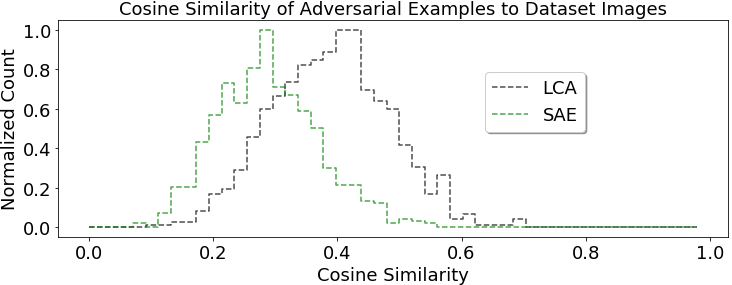
\includegraphics[width=\columnwidth]{Figures/cosyne_similarity.png}}
\end{center}
%\vskip -0.3in
\caption{Adversarial attacks using gradients from the LCA have a larger cosine similarity to dataset images than attacks for the SAE. Following \parencite{kos2018adversarial}, we attacked each model using a target image that was an alternate image from the dataset. The histograms are computed over 800 image examples.}
\end{figure}

To understand how adversarial attacks transfer between these models, we produced adversarial images for each one and test how adversaries generated for one model affect another. The data-aligned perturbations can explain why adversarial images for LCA transfer to SAE and VAE but not the other way around \ref{fig:figure}.

\subsection{Pixel classification attack}
The standard attack method for classification networks is to perturb input pixels to result in misclassification. One proposed defense against this type of attack is to preprocess the image pixels with a denoising autoencoder that would produce reconstructions void of the adversarial pixel perturbations. However, it has been shown that if one backpropagates the adversarial loss through the autoencoder network, then it is still possible to adversarially attack the network. Here we show that the LCA model outperforms the VAE and SAE networks as a preprocessing \"firewall\" against the adversarial attacks.

\subsection{Generative adversarial attacks}
Recent results from \citet{kos2018adversarial} show that adversarial stimulus can be constructed for generative models. This is especially compelling because generative models are explicitly trained to preserve information about the input and produce a veridical reconstruction, whereas classification networks are typically trained to throw away large amounts of information and only preserve that which is relevant for the given task. We show that the LCA model is robust against generative adversarial attacks when compared to the SAE and VAE networks.

%
% * best solution is identity, but that is not an interesting solution
% * this attack prefers simpler models
% * which is why we include sae w/ tied weights
%

\begin{figure}[h]\label{fig:kos_attack}
%\vskip -0.05in
\begin{center}
\centerline{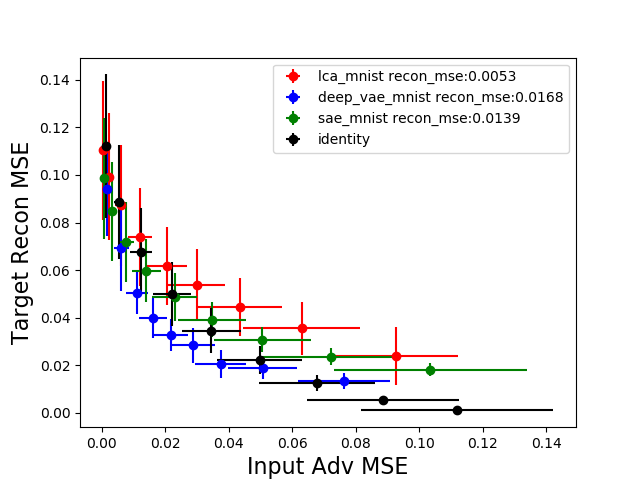
\includegraphics[width=\columnwidth]{Figures/recon_mult_tradeoff.png}}
\end{center}
%\vskip -0.3in
\caption{TODO}
\end{figure}

\subsection{Latent classification attack}
The lateral connectivity in the LCA network is utilized via a recurrent computation. These dynamics facilitate a form of explaining away, where neurons that have a high degree of correspondence with the input stimulus suppress other neurons in the network. This results in the network ignoring input pixels that are not aligned with primary data directions. To better understand the role of the recurrent computation, we trained a network that acts as an unrolled version of LCA, where the lateral connectivity and feedforward weight matrices are learned. The LISTA model was demonstrated by Gregor et al. \citeyearpar{gregor2010learning} to show that a network with many fewer inference steps can produce codes that have a small Euclidean distance to the outputs of sparse coding. We trained three LISTA models with 5, 20, and 50 layers. All three models were trained to produce codes that had approximately the same $L_{2}$ distance from the codes produced by LCA. We show that the LISTA network does not perform as well as LCA at defending against adversarial attacks and that the deeper LISTA networks perform better.

\begin{figure}[h]
\vskip -0.05in
  \begin{subfigure}
    \centering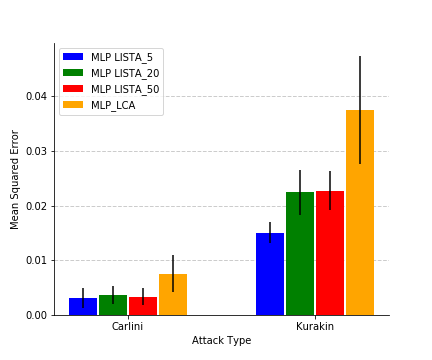
\includegraphics[width=\columnwidth]{Figures/latent_clf_attack_mse.png}
  \end{subfigure}
  \begin{subfigure}
    \centering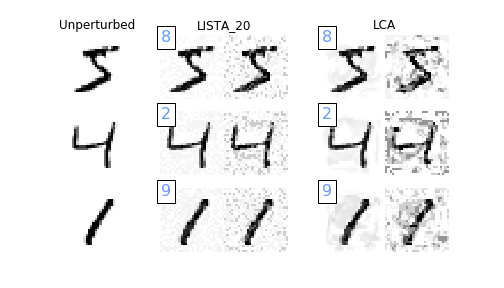
\includegraphics[width=\columnwidth]{Figures/latent_clf_attack_ex.png}
  \end{subfigure}
\caption{LCA better protects against latent classification attacks. We generated adversarial examples from equal-sized MLPs trained from the latent codes of each model. MSEs were calculated between the original image and the perturbed image.   Error bars indicate standard deviation for 100 example inputs.}
\label{fig:latent_attac_mse}
\end{figure}

\subsection{Attacks with the CIFAR dataset}
The LCA objective is derived from a model of natural images, so we believe the network will exhibit stronger aversion to adversarial perturbations.
%%%% From paper

\section{Explaining increased orientation selectivity}
A longstanding hypothesis in visual neuroscience is that sensory neurons are adapted to natural image statistics to produce an efficient code. Independent Component Analysis (ICA) has been proposed as a normative model for simple cells in V1 based on its ability to reduce higher-order redundancy in natural images. When applied to natural images, the filters that emerge resemble the localized, oriented, and band-pass receptive fields of V1 neurons. However, quantitative analyses of the coding efficiency of ICA show that the neural code it produces fails to provide any appreciable gain in redundancy reduction beyond second-order methods such as PCA. This result appears to challenge the higher-order redundancy reduction account of V1 function. We explain these findings by distinguishing oriented filters from orientation \textit{selectivity} and show that ICA's linear encoding scheme fails to implement genuine orientation selectivity, which limits its capacity to learn an efficient code. We show that sparse coding, a related model with a nonlinear encoding scheme that produces orientation selective neurons, is able to achieve a more efficient code than both ICA and PCA when evaluated in the rate-distortion framework, thus providing renewed support for the efficient coding account of V1 receptive field properties.

A long-standing hypothesis in sensory neuroscience proposes that a primary function of early sensory processing is to form an efficient, redundancy-reduced code of the input that maximizes the brain's limited computational and biological resources while making explicit the statistical structure of the input \parencite{barlow2001redundancy}. This hypothesis predicts that the response properties of sensory neurons should be adapted to the statistical structure of their input.

In support of this hypothesis, a number of the response properties of visual neurons have been reproduced by optimizing redundancy-reducing linear transformations on natural images \parencite{atick1990towards}. For example, a symmetric decorrelation transformation of natural images yields center-surround receptive fields \parencite{atick1990towards}, and Principal Component Analysis (PCA) applied to color images yields the luminance, red-green, and blue-yellow channel observed in the opponent color coding of retinal ganglion cells \parencite{ruderman1998statistics, buchsbaum1983trichromacy}. When higher-order correlations are additionally reduced, localized and oriented band-pass filters that resemble the orientation-selective receptive fields in V1 emerge \parencite{bell1997independent, olshausen1999probabilistic}. It has thus been proposed that the oriented filters in V1 function to remove higher-order correlations.

Orientation selectivity is a striking feature of the response properties of simple cells in V1. Since the discovery of orientation selectivity in Hubel and Wiesel's Nobel Prize-winning work, the mechanism for the computation has remained unclear. A common point of confusion in the field has been the assumption that a neuron with an locally oriented receptive field will exhibit orientation selectivity. Here, we will argue that orientation selectivity requires a non-linear encoding process in addition to an oriented receptive field.

Independent Component Analysis (ICA) is one of the most widely used image coding algorithms and has been proposed as a model for simple cells in V1 \parencite{bell1997independent}. The ICA algorithm explicitly optimizes for higher-order redundancy reduction, aiming to to reconstruct the input image as a linear superposition of a set of basis functions while minimizing the mutual information between those bases.

\citeit{eichhorn2009natural} compare the  coding efficiency of ICA and PCA to obtain the surprising result that ICA performs no better than PCA on a rate-distortion trade-off metric. ICA is trained with the objective of minimizing the joint entropy of the activations and learns oriented filters that suggest it has succeeded in modeling higher-order pixel correlations, while PCA is a second-order method that does not learn oriented filters. \citeit{eichhorn2009natural} argue that if ICA had succeeded at capturing higher-order statistics, it should show an advantage in the rate-distortion trade-off.

We present an alternate explanation of these findings by distinguishing \textit{orientation selectivity} from \textit{oriented filters}. Neurons achieve orientation selectivity via a fundamentally nonlinear process, as exhibited by nonclassical receptive field (nCRF) effects such as cross-orientation suppression \parencite{golden2016conjectures, zhu2013visual}. We argue that although the ICA optimization algorithm is able to learn oriented filters, ICA's linear encoding process limits its capacity to perform genuine orientation selectivity, which in turn limits its capacity to produce an efficient code. \citeit{zhu2013visual} demonstrate that sparse coding is able to provide a parsimonious explanation of both classical and nonclassical receptive field properties using a neural network implementing sparse coding \parencite{zhu2013visual}. Here, we replicate the rate-distortion analyses from \citeit{eichhorn2009natural} using the sparse coding network described by \citeit{zhu2013visual} to show that a nonlinear encoding process produces more efficient codes to linear encoders. To assess the degree of orientation selectivity for ICA neurons, we replicate the cross-orientation suppression experiment performed by \citeit{zhu2013visual} with both sparse coding and ICA networks.


\subsection{Rate-distortion analyses}
The Shannon standard for evaluating the efficiency of lossy continuous codes is the rate-distortion framework \parencite{cover2012elements}. \citeit{eichhorn2009natural} compare the  coding efficiency of ICA and PCA and find that PCA performs \textit{better} than ICA in terms of the rate-distortion trade-off. This result is surprising in that ICA is explicitly trained with the goal of minimizing the joint entropy of the activations and learns oriented filters that would suggest that it achieved the goal of modeling higher-order correlations, while PCA is a second-order method that does not learn oriented filters.

We resolve this apparent paradox by distinguishing \textit{orientation selectivity} and \textit{oriented filters}. Neurons achieve orientation selectivity via a fundamentally non-linear process, as exhibited by non-classical receptive field (nCRF) effects such as contrast invariant tuning and cross-orientation suppression \parencite{ferster2000natural,  zhu2013visual}. We argue that although the ICA optimization algorithm is able to learn oriented filters, ICA's linear encoding process limits its capacity to perform genuine orientation selectivity, which in turn limits its capacity to produce an efficient code. Sparse coding is unique in its ability to provide a parsimonious explanation of both classical and non-classical receptive field properties \parencite{zhu2013visual, golden2016conjectures}. Although nCRF effects are typically modeled individually, \citeit{zhu2013visual} show that a wide variety of these effects are emergent properties of a neural network implementing sparse coding. * something about LCA * These findings suggests the primacy of efficient coding in V1. This explanation only holds, however, if sparse coding can be quantitatively shown to achieve a gain in coding efficiency beyond second-order methods. Here, we replicate the rate-distortion analyses from \citeit{eichhorn2009natural} and show that sparse coding's non-linear encoding process enables codes that are lower entropy than those learned by ICA or PCA while being more perceptually robust to increasingly coarse quantization.


\subsection{Methods and Results}
We train sparse coding \parencite{rozell2008sparse}, ICA \parencite{bell1997independent}, and PCA on 1 million 16 x 16 pixel grayscale image patches extracted from images in the van Hateren dataset of natural scenes, which have been transformed to log intensity and standardized to zero mean and unit variance \parencite{vanHateren1998independent}. Using the learned filter matrices, we compute model activations for a test set of 100,000 patches and uniformly quantize these activations with varying degrees of granularity. For each level of granularity, we compute a reconstruction of the test input using the quantized activations and compute the mean squared error. Figure \ref{fig:rd_curve} plots the rate (mean marginal discrete entropy of the activations) against the distortion (mean squared error).

%\begin{figure}[ht]
%\vskip 0.1in
% \centering \includegraphics[width=\linewidth]{figures/rd_curves.png}
% \caption{Discrete entropy vs. reconstruction error for sparse coding, PCA, and ICA.}
%\vskip -0.2in
%\label{fig:rd_curve}
%\end{figure}

Results for sparse coding models trained with different values of $\lambda$ are shown, where a larger $\lambda$ indicates higher sparsity. We replicate the findings from \citeit{eichhorn2009natural} that (orthogonal) PCA  performs slightly better than ICA in the rate-distortion trade-off. Sparse coding shows an advantage over both ICA and PCA. Additionally, we find that representations that are more sparse are capable of achieving increasingly lower rates.
Figure \ref{fig:recons} shows an example reconstruction in the highly lossy (low entropy) regime. For a mean marginal entropy of $H\approx 0.4$, sparse coding shows an advantage in perceptual quality, as well as a quantitative advantage in terms of mean squared error.

%\begin{figure}[ht]
%\vskip 0.1in
% \centering
% \includegraphics[width=\linewidth]{figures/baboon_4_square.png}
% \caption{Lossy reconstructions for quantized activations with mean marginal entropy $H\approx 0.4$}
%\vskip -0.2in
%\label{fig:recons}
%\end{figure}


\subsection{Discussion}
Our results suggest the importance of nonlinear encoding for learning efficient codes of natural images and demonstrate that orientation \textit{selective} neurons are capable of reducing higher-order redundancy. We show that although the ICA algorithm is able to learn oriented filters, ICA's linear encoding process limits its capacity to perform genuine orientation selectivity, which in turn limits its capacity to produce an efficient code. 

Although sparse coding produces a more efficient representation of natural image and neurons that have a higher degree of orientation selectivity than ICA, the model is nonetheless fundamentally limited in its capacity to fully characterize the statistics of natural scenes because it assumes a linear generative model and the light that forms images is combined in a non-linear fashion, such as by occlusion. In future work we plan to extend our analysis to hierarchical models of natural scenes that may achieve greater gains in coding efficiency.

The efficient coding hypothesis was initially posed in terms of redundancy reduction \parencite{barlow1961possible}, under the hypothesis that the brain may seek an efficient code of the input in order to minimize the number of neurons required to represent the signal. Anatomical evidence tells us, however, that the V1 expands the image representation coming from LGN by having many more outputs than inputs \parencite{olshausen2003principles} Thus, redundancies are actually \textit{created} in the perceptual process. The goal of cortical processing, then, cannot be said to be redundancy reduction and simple compression.

As an alternative, several researchers have argued that the goal of perception cannot be discussed in isolation from action; an organism forms perceptual representations for the purpose of directing its behavior towards the achievement of desirable outcomes and away from undesirable ones \parencite{barlow2001redundancy, simoncelli2001natural}. From this perspective, the brain aims to extract the statistical structure of the input in order to form a``meaningful'' representation that recovers the environmental causes of the sensory data, which it can use to guide action. Along these lines, the efficient coding hypothesis has been revised to emphasize redundancy \textit{representation} rather than reduction \parencite{barlow2001redundancy}. Redundancies in the input signal indicate structure in the environment. An encoding that makes these redundancies explicit encodes the causal and statistical structure of the environment, which the organism can exploit to plan and direct behavior.

Sparse coding performs redundancy representation rather than redundancy reduction. A sparse code is a highly redundant code It has been demonstrated that a typical redundancy reducing code--which would form a distributed representation of the input with a high activity ratio--would actually lead to large errors in estimates of the frequency of a particular input, since many neurons are active in response to both the input of interest as well as other stimuli \parencite{gardnermedwin2001limits}. A sparse code, in which the elements of the learned dictionary occur independently in the environment, is a factorial code; the probability of any composite image is simply the product of the probabilities of the components. Any deviations from this rule signal a previously unknown statistical dependency to be learned.

 An efficient code exploits the redundancies in the input signal. The objective of early sensory processing was initially described as redundancy reduction. The redundancy reduction hypothesis was partially motivated by the observation that a significant information bottleneck exists in the first stage of visual processing; most mammals have vastly more photoreceptors than fibers in the optic nerve, which suggests that significant compression must occur in the first stage of processing. However, at moderate to high luminance levels, only a small subset of the photoreceptors are operating within their dynamic ranges; thus the reduction in capacity may be smaller than initially implied. Further, beyond the optic nerve, the number of neurons involved in subsequent layers of processing generally increases, which means that redundancies are actually created in the perceptual process. The goal of early vision, then, cannot be said to be redundancy reduction. From a functional standpoint, several researchers have also argued that the goal of perception is not simple compression; an organism forms perceptual representations in order to direct its behavior towards the achievement of desirable outcomes and away from undesirable ones \parencite{barlow2001redundancy, simoncelli2001natural}. From this standpoint, one can argue that brain aims to extract the statistical structure of the input in order to form a \textit{meaningful} representation that recovers the environmental causes of the sensory data, which it can use to guide action.
 
 Along these lines, the efficient coding hypothesis has been revised more recently to emphasize redundancy representation rather than reduction \parencite{barlow2001redundancy}. Redundancies in the input signal indicate structure in the environment. An encoding that makes these redundancies explicit encodes the causal and statistical structure of the environment, which the organism can exploit to plan and direct behavior. Barlow further argues that to facilitate the identification of the statistics of the environment, neural responses should form a sparse code of the input. He notes that a typical redundancy-reducing code would be a distributed representation of the input with a high activity ratio–that is, a large percentage of active neurons, each of which is frequently active across different inputs. Such a code will lead to large errors in estimates of the frequency of a particular input, since many neurons are active in response to both the input of interest as well as other stimuli. A sparse code, in which the elements of the learned dictionary occur independently in the environment, would form a factorial code, in which the probability of any composite image is simply the product of the probabilities of the components. Any deviations from this rule would signal a previously unknown statistical dependency to be learned.
 
%%%% From paper
Although the softmax nonlinearity used in most classification models is a population nonlinearity, we hypothesize that an adversarial image perturbation can produce adversarial inputs to the softmax, negating it's ability to protect the network against the attack.

Additional control models need to be explored, including alternative population nonlinearities such as those present in Boltzmann machines \parencite{salakhutdinov2009deep}, divisive normalization \parencite{balle2016end}, and local response normalization \parencite{krizhevsky2012imagenet}. Each of these nonlinearities has had significance in the deep learning and neuroscience communities. The iso-response analysis provides a methodology for contrasting them and will give us valuable insight into how each of them may respond to adversarial attacks. We also wish to scale up the models to include larger datasets of more naturalistic images. 

Hierarchical extensions to the sparse coding model \parencite{chen2018sparse} have been shown by our group to perform a better job of mapping input data onto a smooth manifold. We hypothesize that this will further increase the semantic relevance and model robustness for adversarial perturbations. We intend to include the model defined in \parencite{chen2018sparse} in our future analysis to explore how the adversarial and iso-response properties change as we increase the network depth.

This methodology has a high potential for impact in the deep learning community. We advocate for biologically motivated computations that go beyond the simple pointwise nonlinear model. We have shown that these types of networks learn a more robust representation of data without tedious and biased human labeling. We also provide strong theoretical support for our hypotheses and an analysis method that allows us to fully characterize how the more complicated neurons will respond to input perturbations.
%%%%

\section{Explaining extra-classical receptive field effects}
Golden, explaining others.


\section{Applications to physiological neuroscience}
Use this method to probe neuron contours.